\chapter{Comparaci\'on de algoritmos}

\section{Tiempo de ejecuci\'on}

\subsection{Dijkstra}
\begin{table}[H]
\label{tablax}
\begin{center}
\begin{tabular}{|c|c|c|c|}
\hline 
 &32b&16b&8b \\
\hline
1 & 210$\mu s$ & 67$\mu s$ & 123$\mu s$ \\ \hline
2& 208$\mu s$& 149$\mu s$ & 66$\mu s$ \\ \hline
3& 237$\mu s$ & 63$\mu s$ & 66$\mu s$ \\ \hline
4& 208$\mu s$ & 51$\mu s$ & 49$\mu s$ \\ \hline
5& 235$\mu s$ & 106$\mu s$ & 57$\mu s$ \\ \hline
6&209$\mu s$ & 51$\mu s$ & 62$\mu s$ \\ \hline
7& 206$\mu s$ & 74$\mu s$ & 70$\mu s$ \\ \hline
8&235$\mu s$ & 46$\mu s$ & 141$\mu s$ \\ \hline
9& 203$\mu s$ & 50$\mu s$ & 47$\mu s$ \\ \hline
10& 206$\mu s$ & 47$\mu s$ & 57$\mu s$ \\ \hline
\end{tabular}
\end{center}
\caption{Eficiencia en ejecuci\'on}
\end{table}

\subsection{Euclides Clasico}
\begin{table}[H]
\label{tablax}
\begin{center}
\begin{tabular}{|c|c|c|c|}
\hline 
 &32b&16b&8b \\
\hline
1 & 195$\mu s$ & 193$\mu s$ & 228$\mu s$ \\ \hline
2& 1981$\mu s$& 271$\mu s$ & 231$\mu s$ \\ \hline
3& 587$\mu s$ & 596$\mu s$ & 226$\mu s$ \\ \hline
4& 213$\mu s$ & 210$\mu s$ & 223$\mu s$ \\ \hline
5& 621$\mu s$ & 601$\mu s$ & 225$\mu s$ \\ \hline
6& 218$\mu s$ & 213$\mu s$ & 229$\mu s$ \\ \hline
7& 214$\mu s$ & 186$\mu s$ & 217$\mu s$ \\ \hline
8& 552$\mu s$ & 219$\mu s$ & 210$\mu s$ \\ \hline
9& 550$\mu s$ & 205$\mu s$ & 211$\mu s$ \\ \hline
10& 561$\mu s$ & 213$\mu s$ & 219$\mu s$ \\ \hline
\end{tabular}
\end{center}
\caption{Eficiencia de ejecuci\'on}
\end{table}

\subsection{Binario Euclides}
\begin{table}[H]
\label{tablax}
\begin{center}
\begin{tabular}{|c|c|c|c|}
\hline 
 &32b&16b&8b \\
\hline
1 & 232$\mu s$ & 604$\mu s$ & 220$\mu s$ \\ \hline
2& 582$\mu s$& 572$\mu s$ & 224$\mu s$ \\ \hline
3& 644$\mu s$ & 608$\mu s$ & 576$\mu s$ \\ \hline
4& 224$\mu s$ & 212$\mu s$ & 220$\mu s$ \\ \hline
5& 228$\mu s$ & 225$\mu s$ & 608$\mu s$ \\ \hline
6& 203$\mu s$ & 217$\mu s$ & 219$\mu s$ \\ \hline
7& 229$\mu s$ & 211$\mu s$ & 619$\mu s$ \\ \hline
8& 228$\mu s$ & 220$\mu s$ & 694$\mu s$ \\ \hline
9& 206$\mu s$ & 218$\mu s$ & 612$\mu s$ \\ \hline
10& 579$\mu s$ & 567$\mu s$ & 218$\mu s$ \\ \hline
\end{tabular}
\end{center}
\caption{Eficiencia de ejecuci\'on}
\end{table}

\subsection{Euclides extendido}
\begin{table}[H]
\label{tablax}
\begin{center}
\begin{tabular}{|c|c|c|c|}
\hline 
 &32b&16b&8b \\
\hline
1 & 195$\mu s$ & 180$\mu s$ & 234$\mu s$ \\ \hline
2& 167$\mu s$& 145$\mu s$ & 168$\mu s$ \\ \hline
3& 157$\mu s$ & 147$\mu s$ & 178$\mu s$ \\ \hline
4& 205$\mu s$ & 175$\mu s$ & 157$\mu s$ \\ \hline
5& 169$\mu s$ & 228$\mu s$ & 148$\mu s$ \\ \hline
6& 163$\mu s$ & 146$\mu s$ & 167$\mu s$ \\ \hline
7& 172$\mu s$ & 154$\mu s$ & 175$\mu s$ \\ \hline
8& 191$\mu s$ & 182$\mu s$ & 190$\mu s$ \\ \hline
9& 172$\mu s$ & 178$\mu s$ & 175$\mu s$ \\ \hline
10& 168$\mu s$ & 163$\mu s$ & 171$\mu s$ \\ \hline
\end{tabular}
\end{center}
\caption{Eficiencia de ejecuci\'on}
\end{table}

\subsection{Lehmer GCD}
\begin{table}[H]
\label{tablax}
\begin{center}
\begin{tabular}{|c|c|c|c|}
\hline 
 &32b&16b&8b \\
\hline
1 & 642$\mu s$ & 484$\mu s$ & 440$\mu s$ \\ \hline
2& 1077$\mu s$& 964$\mu s$ & 530$\mu s$ \\ \hline
3& 1135$\mu s$ & 461$\mu s$ & 537$\mu s$ \\ \hline
4& 624$\mu s$ & 803$\mu s$ & 557$\mu s$ \\ \hline
5& 640$\mu s$ & 467$\mu s$ & 453$\mu s$ \\ \hline
6& 676$\mu s$ & 465$\mu s$ & 449$\mu s$ \\ \hline
7& 696$\mu s$ & 491$\mu s$ & 948$\mu s$ \\ \hline
8& 621$\mu s$ & 474$\mu s$ & 2261$\mu s$ \\ \hline
9& 609$\mu s$ & 468$\mu s$ & 441$\mu s$ \\ \hline
10& 1168$\mu s$ & 456$\mu s$ & 447$\mu s$ \\ \hline
\end{tabular}
\end{center}
\caption{Eficiencia de ejecuci\'on}
\end{table}

\begin{figure}[H]
 \centering
 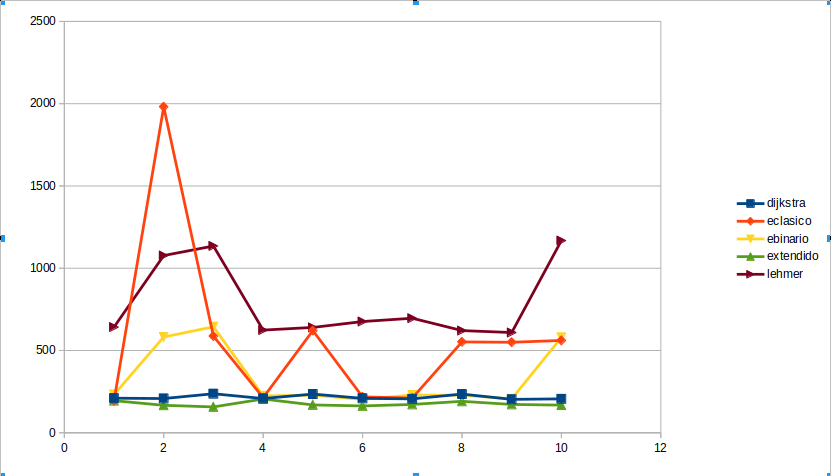
\includegraphics[scale=0.4]{./32bits.png}
 % 32bits.png: 0x0 pixel, 300dpi, 0.00x0.00 cm, bb=
 \caption{Tiempo de ejecución de 32-Bits}
 \label{fig:1}
\end{figure}



\section{Convergencia}

\begin{table}[H]
\label{tablax}
\begin{center}
\begin{tabular}{|c|c|c|c|}
\hline 
 &32b&16b&8b \\
\hline
Dijkstra& 17 & 8 & 8 \\ \hline
E. Clasico& 17& 8 & 8 \\ \hline
E. Binario& 36 & 21 & 12 \\ \hline
E. Extendido& 17 & 8 & 8 \\ \hline
Lehmer& 24 & 24 & 24 \\ \hline
\end{tabular}
\end{center}
\caption{Numero de iteraciones por algoritmos}
\end{table}

\begin{figure}[h]
 \centering
 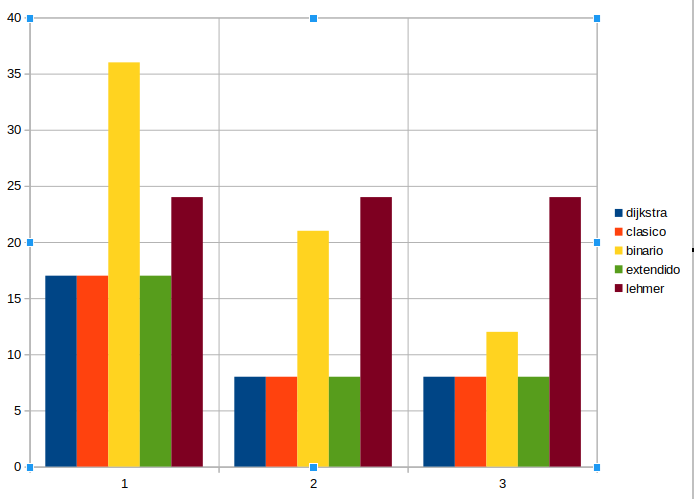
\includegraphics[scale=0.4]{./iteracion.png}
 % iteracion.png: 0x0 pixel, 300dpi, 0.00x0.00 cm, bb=
 \caption{Nro de Iteraciones en 32, 16 y 8 bits}
 \label{fig:2}
\end{figure}


\section{Acumulaci\'on de variables}

\begin{table}[H]
\label{tablax}
\begin{center}
\begin{tabular}{|c|c|c|c|}
\hline 
 &32b&16b&8b \\
\hline
Dijkstra& 50 & 50 & 50 \\ \hline
E. Clasico& 44 & 44 & 44 \\ \hline
E. Binario& 5 & 5 & 5 \\ \hline
E. Extendido& 10 & 10 & 10 \\ \hline
Lehmer& 23 & 23 & 23 \\ \hline
\end{tabular}
\end{center}
\caption{Acumulaci\'on de variables por algoritmos}
\end{table}


\begin{figure}[h]
 \centering
 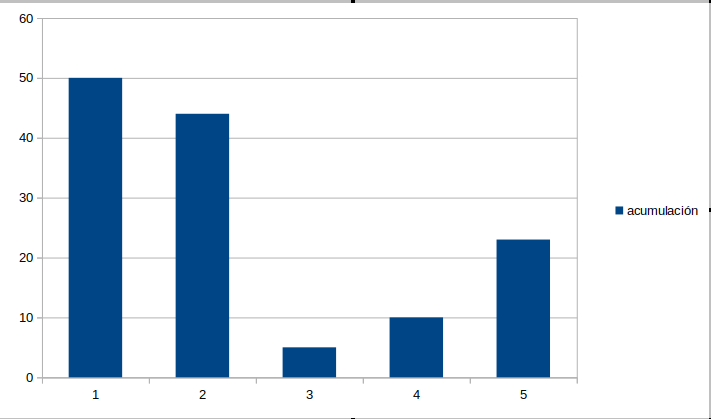
\includegraphics[scale=0.4]{./acmulac.png}
 % acmulac.png: 0x0 pixel, 300dpi, 0.00x0.00 cm, bb=
 \caption{Acumulación de variable de todos los algoritmos}
 \label{fig:3}
\end{figure}

